% =============================================================
% Rascunho da seção de Resultados (Hipóteses H2 e H3 -- topologia do
% gate) para inclusão no artigo final de pgsg_2 (formato elsarticle,
% periódico-alvo Chemolab).
%
% FRAGMENTO -- não compila sozinho. \input{} dentro de \section{Results},
% em sequência a resultados_H1_v2.tex.
%
% Dados-fonte (27-28/07/2026):
%   scripts/run_h1_raman_v2.py        -> h1_raman_v2_result.npz (Raman)
%   scripts/ablation_h3_smoothness.py -> ablation_h3_result.npz (NIR, prior gaussiano)
%   scripts/extract_nir_gate_v2.py    -> nir_gate_v2_extraction.npz (NIR, prior degrau original)
%   scripts/reanalyze_smoothness_physical.py -> normalização por cm-1
% Figura: h2h3_topology.pdf
% =============================================================

\subsection{H2 e H3: Topologia do gate entre modalidades}
\label{sec:results-h2h3}

As Hipóteses~2 e~3 preveem que a topologia do gate aprendido --- caracterizada pelos descritores formais da Seção~\ref{sec:topologia} --- difere sistematicamente entre NIR e Raman de forma consistente com a física de cada modalidade: gate mais esparso em Raman (picos estreitos) e mais suave em NIR (bandas largas e sobrepostas).

\paragraph{H2 (esparsidade).} Suportada, e robusta à forma de codificação do prior. Com os priors originais de cada modalidade (NIR: função degrau, \texttt{make\_literature\_prior}; Raman: soma de gaussianas), a esparsidade de Hoyer é $S_{\text{NIR}}=0{,}3176$ vs.\ $S_{\text{Raman}}=0{,}4150$. Controlando a forma funcional (recodificando o prior NIR como gaussianas, mesmo estilo do Raman --- Seção~\ref{sec:ablation}), a diferença se mantém e até aumenta: $S_{\text{NIR}}=0{,}2345$ vs.\ $S_{\text{Raman}}=0{,}4150$ (Figura~\ref{fig:h2h3-topology}a). Raman produz gates mais concentrados em poucas bandas do que NIR, na direção prevista.

\paragraph{H3 (suavidade) --- confundidor identificado e resolvido.} Uma primeira comparação, usando a variação total por \emph{índice de banda} (Seção~\ref{sec:topologia}, fórmula original), produziu o resultado \emph{oposto} ao previsto: $\mathrm{TV}_{\text{NIR}}=0{,}016692 > \mathrm{TV}_{\text{Raman}}=0{,}007570$ (Figura~\ref{fig:h2h3-topology}b), sugerindo NIR menos suave que Raman. Esse resultado persistiu mesmo controlando a forma funcional do prior (Seção~\ref{sec:ablation}), descartando a codificação do prior como causa.

A causa real é uma diferença de \emph{densidade de amostragem espectral} entre as duas modalidades, não uma diferença física de suavidade: o eixo NIR ($p=281$ bandas cobrindo $\approx 26.755$~cm$^{-1}$, $\approx 95$~cm$^{-1}$/banda) é quase 60$\times$ mais esparso, em número de onda, do que o eixo Raman ($p=1.870$ bandas cobrindo $\approx 2.995$~cm$^{-1}$, $\approx 1{,}6$~cm$^{-1}$/banda). A variação total por \emph{índice} confunde "quantas bandas separam duas regiões informativas" com "quão suave é a transição por unidade física de espectro" --- métrica inadequada para comparação entre modalidades com densidades de banda tão distintas.

Recalculando a suavidade por \emph{unidade física} (variação do gate por cm$^{-1}$, convertendo o eixo NIR de nm via $\tilde\nu = 10^7/\lambda$), a direção se inverte e passa a corresponder à hipótese original: $\mathrm{TV}_{\text{física,NIR}}=0{,}000369 \ll \mathrm{TV}_{\text{física,Raman}}=0{,}003795$ (Figura~\ref{fig:h2h3-topology}c). Esse resultado converge com uma verificação totalmente independente --- a suavidade do \emph{espectro bruto} pré-processado, sem qualquer gate ou prior envolvido --- que mostra o mesmo padrão: o espectro Raman é $\approx 2{,}3\times$ mais "áspero" (variação ponto-a-ponto maior) do que o espectro NIR ($0{,}2156$ vs.\ $0{,}0926$). Duas medidas independentes, uma derivada do gate aprendido e outra do dado bruto, concordam: \textbf{H3 é suportada}, desde que a suavidade seja medida corretamente por unidade física de espectro, não por índice bruto de banda.

\begin{figure}[htbp]
    \centering
    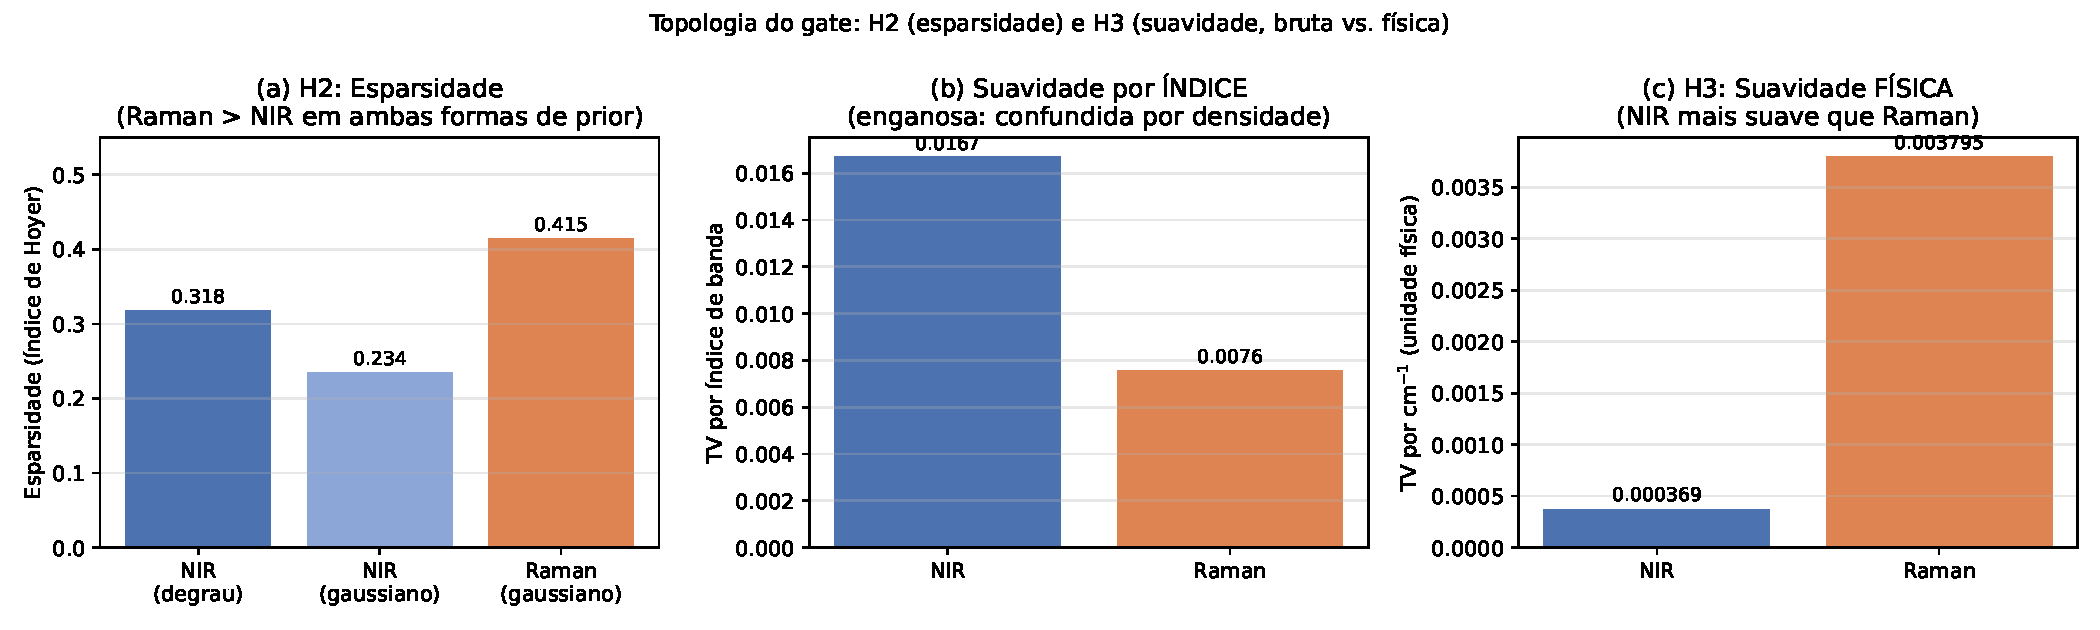
\includegraphics[width=\linewidth]{h2h3_topology.pdf}
    \caption{Topologia do gate entre modalidades. (a) Esparsidade de Hoyer: Raman mais esparso que NIR, com ambas as formas de prior. (b) Suavidade por índice de banda: direção enganosa, dominada pela diferença de densidade espectral entre modalidades. (c) Suavidade por unidade física (cm$^{-1}$): direção correta, convergente com a suavidade do espectro bruto -- NIR mais suave, Raman mais "áspero".}
    \label{fig:h2h3-topology}
\end{figure}

\subsection{Ablação: forma funcional do prior}
\label{sec:ablation}

Como $\rho(g,s)$ é muito alto em ambas as modalidades (Seção~\ref{sec:results-h1}: $0{,}998$ em NIR, $0{,}978$ em Raman), a topologia do gate final herda em grande parte a topologia do \emph{prior} de inicialização. Isso levanta um confundidor metodológico: o prior NIR oficial (\texttt{make\_literature\_prior}) é uma função degrau (patamares constantes, saltos abruptos nas fronteiras de região), enquanto o prior Raman (Seção de priors) é uma soma de gaussianas suaves --- formas funcionais diferentes que, por si só, poderiam gerar diferenças de topologia sem relação com a física da modalidade.

Para isolar esse efeito, o prior NIR foi recodificado como soma de gaussianas (mesmos centros e pesos relativos de \texttt{make\_literature\_prior}: 690~nm, peso 0,6; 950~nm, peso 1,0; 1150~nm, peso 0,8), e o \texttt{PGSGv2Model} foi retreinado sob essa nova inicialização --- sem qualquer outra alteração. O desempenho preditivo permanece equivalente ($R^2_{\text{PGSGv2}}=0{,}8203$ com prior gaussiano vs.\ $0{,}8128$ com prior degrau, mesmo $R^2_{\text{PLS}}=0{,}5684$), e a direção de H2 se mantém (e se acentua). Isso confirma que as diferenças reportadas acima não são artefato da forma de codificação do prior.

